\documentclass[10pt]{beamer}
\usepackage[nosetup]{evan}
\usetheme{Goddard}

\begin{document}
\title{Thoughts and Q/A on math olympiad coaching}
\subtitle{}
\institute{Excellence in Coaching and Leadership Program \\ Global Talent Network}
\author{Evan Chen}
\date{4 November 2023}

\maketitle

\section{About this sphere}
\begin{frame}
  \frametitle{About this sphere}
  \begin{alertblock}{Bad news}
    Math olympiad coaching is such a small world that
    most things are not written anywhere obvious, if at all.
  \end{alertblock}
  \pause
  Examples of \emph{oral traditions}:
  \begin{itemize}
    \ii No official syllabus of IMO topics exists (unlike IOI).
    \ii Haphazard voting process for problem selection.
    \ii How IMO coordination works (e.g.\ past rubrics).
    \ii What the IMO Shortlist is and how to use it.
    \ii \url{https://aops.com/community/c13}
  \end{itemize}
  \pause
  \begin{exampleblock}{Good news}
    Most coaches are really nice and you should talk to them.
  \end{exampleblock}
\end{frame}

\section{Two key ingredients}
\begin{frame}
  \frametitle{Two key ingredients}
  I would say the \alert{two most important things} are:
  \begin{itemize}
    \ii Excellent problems and solutions on national competitions (at all levels).
    \ii Building and nurturing a community of students and trainers.
  \end{itemize}
\end{frame}

\section{Problems and solutions}
\begin{frame}
  \frametitle{Problems and solutions}
  \begin{block}{These are the raw materials used by students}
    \begin{itemize}
      \ii Quality of MO's sets it apart from other extracurricular activities.
      \begin{itemize}
        \ii Why MO medalists are heavily recruited.
      \end{itemize}
      \ii Good authors and editors are so valuable that money can't buy them.
      \ii Includes the full pyramid, not just the final team selection test.
      \begin{itemize}
        \ii Develops a talent base, not just top-6 IMO squad.
      \end{itemize}
      % \ii Solutions packet are important, not an afterthought.
      % ^ apparently the other USA staff don't think this is true 🤷
    \end{itemize}
  \end{block}
  \pause
  \begin{exampleblock}{Example: USA {\footnotesize (\url{https://web.evanchen.cc/problems.html})}}
    \begin{itemize}
      \ii Each TST had \alert{6-month selection and review}.
      \ii The earlier round AMC/AIME has \alert{2-year review}.
    \end{itemize}
  \end{exampleblock}
\end{frame}
\begin{frame}
  \frametitle{Where to find problems}
  If your system isn't super-mature, it's likely
  unrealistic to create many original problems, especially at IMO level.
  \begin{alertblock}{IMO Shortlist}
    \begin{itemize}
      \ii Shared resource of 24+ problems a year.
      \ii Security issue, but best-written solutions in town.
    \end{itemize}
  \end{alertblock}
  \pause
  \begin{block}{\url{https://aops.com/community/c13}}
    \begin{center}
      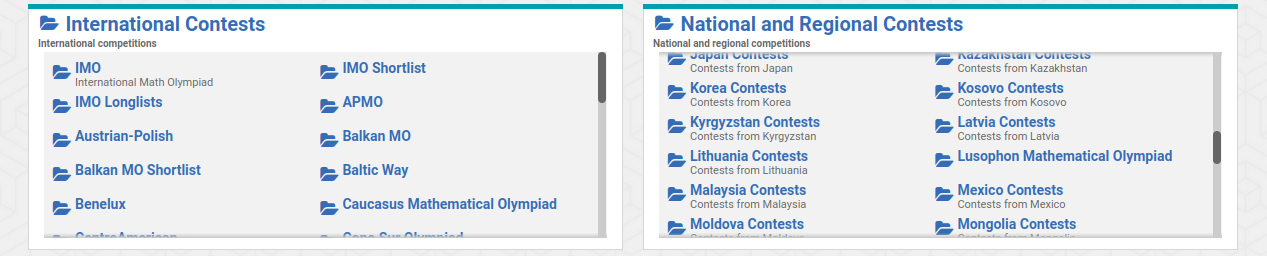
\includegraphics[width=0.8\textwidth]{contest-index.png}
    \end{center}
  \end{block}
  \pause
  \begin{exampleblock}{Collaboration}
    Example: mirrored contests (e.g.\ RMM, APMO).
  \end{exampleblock}
\end{frame}

\section{Community}
\begin{frame}
  \frametitle{Community}
  Building a community out of common interests
  at all levels is super important for talent base.
  \begin{block}{Goals of the human component}
  \begin{itemize}
    \ii Peers to be role models and friends with.
    \ii Space to ask questions, talk about problems, etc.
    \ii Feedback cycle where top students return as trainers and problem proposers
    (reaching escape velocity).
  \end{itemize}
  \end{block}
  \pause
  \begin{exampleblock}{Figure out what students already use and connect them}
    \begin{center}
      
\includegraphics[height=0.5in]{logo-aops.png}
      
\includegraphics[height=0.5in]{logo-whatsapp.png}
      
\includegraphics[height=0.5in]{logo-discord.png}
    \end{center}
  \end{exampleblock}
\end{frame}

\section{Process}
\begin{frame}
  \frametitle{So far\dots}
  \begin{block}{Two stated end-goals}
    \begin{itemize}
      \ii Great problems at all levels build a deep talent base.
      \ii Foster active community based on shared interests.
    \end{itemize}
    How do we get there?
  \end{block}
  \pause
  \begin{alertblock}{Spoiler}
    \begin{itemize}
      \ii It's really hard! (That's why it's interesting.)
      \ii Probably no ``magic bullet'' or one-size-fits-all answer.
      \ii Rather than try to describe a recipe,
      some general advice by showing examples of mistakes I've made.
    \end{itemize}
  \end{alertblock}
\end{frame}
\begin{frame}
  \frametitle{Process}
  \begin{block}{}
    {\slshape
      The most competent people, with weak processes, will screw up.}

    \bigskip \hspace{2em} --- Chris Peterson
  \end{block}
  \begin{block}{}
    {\slshape
      Theory and practice sometimes clash.
      And when that happens, theory loses.
      Every single time.}

    \bigskip \hspace{2em} --- Linus Torvalds
  \end{block}
  \begin{itemize}
    \ii For both goals, pay attention to infrastructure/process.
    \ii Processes must work well in practice, not just in theory.
  \end{itemize}
\end{frame}

\begin{frame}
  \frametitle{Example \#1: college homework model}
  \begin{alertblock}{Failure mode}
    \begin{itemize}
      \ii Used to just send students a PDF of 7 problems,
      ask to solve all of them, and email whenever stuck.
      \ii Led to \textbf{enormous friction}
      whenever student couldn't solve a problem (often).
      \begin{itemize}
        \ii Would often give up on problem or feel discouraged
        \ii Unrealistic \textbf{in practice}
        to expect someone to email Evan every single time
        they can't solve a problem,
        even if it's possible \textbf{in theory}.
      \end{itemize}
    \end{itemize}
  \end{alertblock}
  \pause
  \begin{exampleblock}{Resolution}
    \begin{itemize}
      \ii Point-based problem sets,
      solve any $\binom n7$ or so.
      \ii Large Discord community of peers for discussion.
      \ii Automated pre-written hint system.
    \end{itemize}
  \end{exampleblock}
\end{frame}

\begin{frame}
  \frametitle{Example \#2: USA TST 2014-2017}
  \begin{alertblock}{Failure mode}
    \begin{itemize}
      \ii Haphazard email thread for both proposals and rating,
      with no solutions at all.
      \ii No process to get consensus or organize feedback.
      \ii Unrealistic \textbf{in practice} to expect
      everyone to follow a lot of emails,
      even if it's possible \textbf{in theory}.
    \end{itemize}
  \end{alertblock}
  \pause
  \begin{exampleblock}{Resolution}
    \begin{itemize}
      \ii Created mailing list with clear schedule ahead of time
      (submit problems by X, ratings by Y, test chosen by Z).
      \ii Proposals collated in packet with full solutions.
      \ii Google form to aggregate all ratings and feedback.
    \end{itemize}
  \end{exampleblock}
\end{frame}

\section{Closing}
\begin{frame}
  \frametitle{Closing}
  \begin{block}{Links to these slides and other resources}
    \url{https://web.evanchen.cc/coaches.html}
  \end{block}
  \bigskip
  \pause
  \begin{block}{Most important part of this talk}
    \LARGE\centering Q/A
  \end{block}
\end{frame}

\end{document}
